
%(BEGIN_QUESTION)
% Copyright 2009, Tony R. Kuphaldt, released under the Creative Commons Attribution License (v 1.0)
% This means you may do almost anything with this work of mine, so long as you give me proper credit

Suppose a level measurement system is ``stuck'' at one measurement value of approximately 40\% even when the process liquid level rises and falls between 20\% and 80\% of range (as indicated by the sightglass):

$$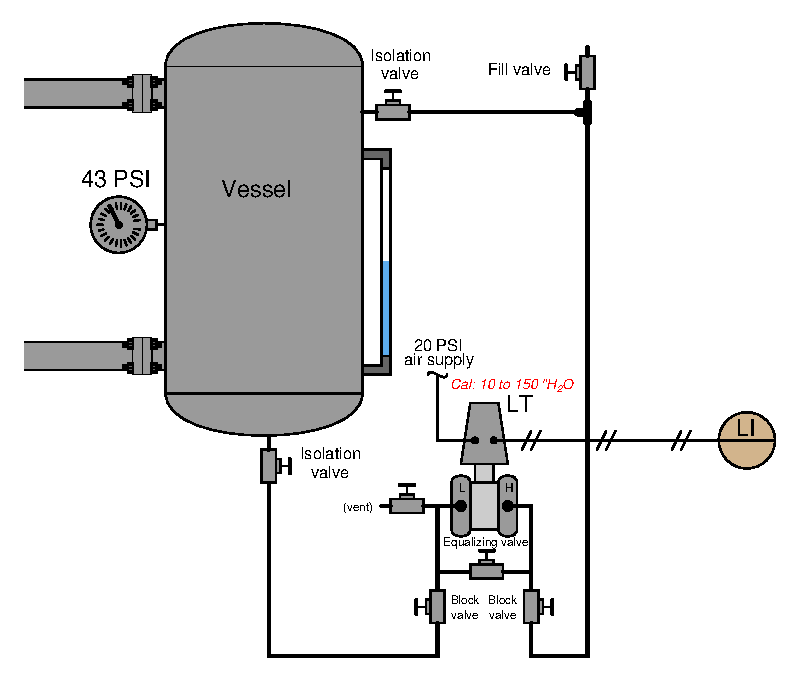
\includegraphics[width=15.5cm]{i00030x01.eps}$$

An instrument technician removes the cover from the pneumatic transmitter and momentarily presses the baffle against the nozzle.  The level indicator in the control room does not respond at all, but remains fixed at about 40\%.

\vskip 10pt

Identify the likelihood of each possible fault in this list by checking boxes in the table -- whether the fault is ``probable'' (worth considering as a cause of this system's trouble) or is ``unlikely'' (either completely ruled out as a cause, or just not worth considering at this point in the diagnosis) -- following the results of the technician's test:

% No blank lines allowed between lines of an \halign structure!
% I use comments (%) instead, so that TeX doesn't choke.

$$\vbox{\offinterlineskip
\halign{\strut
\vrule \quad\hfil # \ \hfil & 
\vrule \quad\hfil # \ \hfil & 
\vrule \quad\hfil # \ \hfil \vrule \cr
\noalign{\hrule}
%
% First row
{\bf Fault} & {\bf Probable} & {\bf Unlikely} \cr
%
\noalign{\hrule}
%
% Another row
Plugged isolation valve &  & \cr
%
\noalign{\hrule}
%
% Another row
Plugged equalizing valve &  & \cr
%
\noalign{\hrule}
%
% Another row
Fill fluid lost in ``wet'' leg &  & \cr
%
\noalign{\hrule}
%
% Another row
Low supply air pressure &  & \cr
%
\noalign{\hrule}
%
% Another row
Transmitter restrictor (orifice) clogged &  & \cr
%
\noalign{\hrule}
%
% Another row
Indicator pointer stuck &  & \cr
%
\noalign{\hrule}
%
% Another row
Transmitter nozzle clogged &  & \cr
%
\noalign{\hrule}
%
% Another row
3-15 PSI signal tubing plugged &  & \cr
%
\noalign{\hrule}
%
% Another row
Transmitter out of calibration &  & \cr
%
\noalign{\hrule}
} % End of \halign 
}$$ % End of \vbox

\vfil 

\underbar{file i00030}
\eject
%(END_QUESTION)





%(BEGIN_ANSWER)

This is a graded question -- no answers or hints given!

%(END_ANSWER)





%(BEGIN_NOTES)

The failed baffle-stimulation test positively indicates a problem somewhere in the pneumatic portion of this system, rather than in the process portion (impulse lines, manifold, etc.).  What we should have seen with the baffle press test is the indicator shoot up past 100\% level.

This means we may reject any of the listed faults that are exclusive to the process, and instead focus on pneumatic component faults.

% No blank lines allowed between lines of an \halign structure!
% I use comments (%) instead, so that TeX doesn't choke.

$$\vbox{\offinterlineskip
\halign{\strut
\vrule \quad\hfil # \ \hfil & 
\vrule \quad\hfil # \ \hfil & 
\vrule \quad\hfil # \ \hfil \vrule \cr
\noalign{\hrule}
%
% First row
{\bf Fault} & {\bf Probable} & {\bf Unlikely} \cr
%
\noalign{\hrule}
%
% Another row
Plugged isolation valve & & $\surd$ \cr
%
\noalign{\hrule}
%
% Another row
Plugged equalizing valve &  & $\surd$ \cr
%
\noalign{\hrule}
%
% Another row
Fill fluid lost in ``wet'' leg &  & $\surd$ \cr
%
\noalign{\hrule}
%
% Another row
Low supply air pressure &  & $\surd$ \cr
%
\noalign{\hrule}
%
% Another row
Transmitter restrictor (orifice) clogged &  & $\surd$ \cr
%
\noalign{\hrule}
%
% Another row
Indicator pointer stuck & $\surd$ & \cr
%
\noalign{\hrule}
%
% Another row
Transmitter nozzle clogged &  & $\surd$ \cr
%
\noalign{\hrule}
%
% Another row
3-15 PSI signal tubing plugged & $\surd$  & \cr
%
\noalign{\hrule}
%
% Another row
Transmitter out of calibration &  & $\surd$ \cr
%
\noalign{\hrule}
} % End of \halign 
}$$ % End of \vbox


%INDEX% Measurement, level: troubleshooting

%(END_NOTES)


